
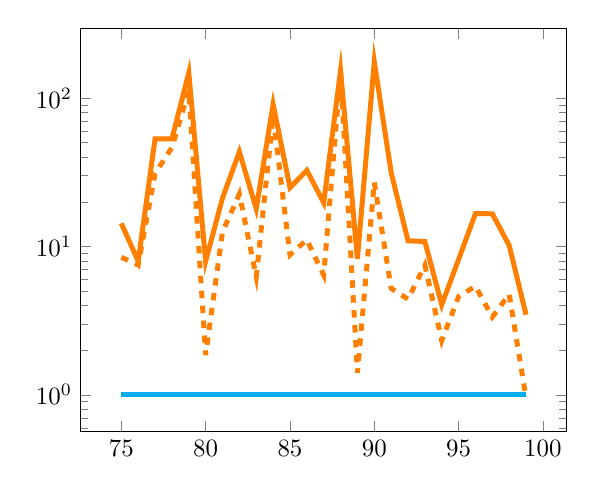
\begin{tikzpicture}[scale=0.9]
\begin{semilogyaxis}
\addplot[color=cyan,line width=2pt,mark options={solid}] coordinates {(75,1.0)(76,1.0)(77,1.0)(78,1.0)(79,1.0)(80,1.0)(81,1.0)(82,1.0)(83,1.0)(84,1.0)(85,1.0)(86,1.0)(87,1.0)(88,1.0)(89,1.0)(90,1.0)(91,1.0)(92,1.0)(93,1.0)(94,1.0)(95,1.0)(96,1.0)(97,1.0)(98,1.0)(99,1.0)};
\addplot[color=orange,line width=2pt,mark options={solid}] coordinates {(75,14.314017562015758)(76,7.945914709608797)(77,53.10268161499488)(78,53.003555917271264)(79,148.0017917890557)(80,7.947710169081388)(81,21.198570067174405)(82,43.44305054813597)(83,17.93184788258092)(84,90.81370231767981)(85,24.907928366671715)(86,32.52417399222413)(87,19.707429209635027)(88,153.2166080642651)(89,8.26865715226)(90,175.50990575651744)(91,31.53096873070394)(92,10.907929360888222)(93,10.800233819917231)(94,4.041643378881029)(95,8.171186976582003)(96,16.670674354975798)(97,16.595258490808565)(98,10.155269389132085)(99,3.463213616684156)};
\addplot[dashed,color=orange,line width=2pt,mark options={solid}] coordinates {(75,8.455855115020078)(76,7.494323508025711)(77,31.058213205733768)(78,46.35692498147781)(79,113.09025044013559)(80,1.8559026802602971)(81,12.534119326749265)(82,22.540861094174407)(83,6.257552277493737)(84,75.88083641227301)(85,8.784677165450118)(86,11.095004549622681)(87,6.41095629502459)(88,150.52657957185093)(89,1.4105348794901198)(90,27.089563957047677)(91,5.217692953291784)(92,4.413390511372132)(93,7.480965014712147)(94,2.3228454983907336)(95,4.60275325858434)(96,5.3944206566625335)(97,3.3451164242636753)(98,4.763652864021808)(99,0.9519949341133745)};

\end{semilogyaxis}
\end{tikzpicture}
